\documentclass[titlepage,twoside,12pt]{book}

%%%%%%%%%%%%%%%%%%%%%%%%%%%%%%%%%%%%%%%%%%%%%%%%%%%%%%%%%%%%%%%%%%%%%%
% Package required for the logical manipulations
%%%%%%%%%%%%%%%%%%%%%%%%%%%%%%%%%%%%%%%%%%%%%%%%%%%%%%%%%%%%%%%%%%%%%%
\usepackage{ifthen}

%%%%%%%%%%%%%%%%%%%%%%%%%%%%%%%%%%%%%%%%%%%%%%%%%%%%%%%%%%%%%%%%%%%%%%
% Structure of the theorems, propositions, ...
%%%%%%%%%%%%%%%%%%%%%%%%%%%%%%%%%%%%%%%%%%%%%%%%%%%%%%%%%%%%%%%%%%%%%%
\usepackage{bm}
\usepackage{amsmath}
\usepackage{amssymb}
\usepackage{amscd}
\usepackage{amsthm}
\usepackage{stmaryrd}

\allowdisplaybreaks

\usepackage[breakable]{tcolorbox}
\tcbuselibrary{skins}

\newcounter{focus}[section]
\renewcommand\thefocus{\thesection.\arabic{focus}}
\newcommand{\focuscolor}{violet}

\makeatletter

\newcommand{\focus@one}[1][RRR]{\def\argfocus@one{#1}\focus@two}

\newcommand{\focus@two}[2][TTT]%
{\refstepcounter{focus}%
  \ifthenelse{\equal{\dfn}{#2}}{\renewcommand{\focuscolor}{purple}}{}%
  \begin{tcolorbox}[enhanced,breakable,colback=\focuscolor!5!white,colframe=\focuscolor!50!white,colbacktitle=\focuscolor!50!white,coltitle=black,drop fuzzy shadow=black!50!white,%
    title={\bfseries #2 \thefocus}%
    \ifthenelse{\equal{TTT}{#1}}{}{\ ({\bfseries #1})}%
    \ifthenelse{\equal{RRR}{\argfocus@one}}{}{\ \argfocus@one}]%
    \renewcommand{\labelitemi}{\textbullet}%
  }

\newenvironment{focus}{\focus@one}{\end{tcolorbox}\renewcommand{\focuscolor}{purple}}

\newcommand{\focusS@one}[1][RRR]{\def\argfocusS@one{#1}\focusS@two}

\newcommand{\focusS@two}[2][TTT]%
{\ifthenelse{\equal{\dfn}{#2}}{\renewcommand{\focuscolor}{purple}}{}%
  \begin{tcolorbox}[enhanced,breakable,colback=\focuscolor!5!white,colframe=\focuscolor!50!white,colbacktitle=\focuscolor!50!white,coltitle=black,drop fuzzy shadow=black!50!white,%
    title={\bfseries #2}%
    \ifthenelse{\equal{TTT}{#1}}{}{\ ({\bfseries #1})}%
    \ifthenelse{\equal{RRR}{\argfocusS@one}}{}{\ \argfocusS@one}]%
    \renewcommand{\labelitemi}{\textbullet}%
  }

\newenvironment{focus*}{\focusS@one}{\end{tcolorbox}\renewcommand{\focuscolor}{purple}}

\makeatother

\newcommand{\dfn}{D\'efiniton}
\newcommand{\prp}{Proposition}
\newcommand{\thm}{Th\'eor\`eme}
\newcommand{\cor}{Corollaire}
\newcommand{\prop}{Proposition}
\newcommand{\lmm}{Lemme}
\newcommand{\mth}{M\'ethode}

%%%%%%%%%%%%%%%%%%%%%%%%%%%%%%%%%%%%%%%%%%%%%%%%%%%%%%%%%%%%%%%%%%%%%%
% If something has to go in the margin
%%%%%%%%%%%%%%%%%%%%%%%%%%%%%%%%%%%%%%%%%%%%%%%%%%%%%%%%%%%%%%%%%%%%%%
\setlength{\oddsidemargin}{0cm}
\setlength{\evensidemargin}{0cm}
\setlength{\marginparwidth}{1.1cm}
\setlength{\marginparsep}{0.5cm}
\reversemarginpar

%%%%%%%%%%%%%%%%%%%%%%%%%%%%%%%%%%%%%%%%%%%%%%%%%%%%%%%%%%%%%%%%%%%%%%
% Counter for the equation number
%%%%%%%%%%%%%%%%%%%%%%%%%%%%%%%%%%%%%%%%%%%%%%%%%%%%%%%%%%%%%%%%%%%%%%
\setcounter{secnumdepth}{2}
\numberwithin{equation}{section}

%%%%%%%%%%%%%%%%%%%%%%%%%%%%%%%%%%%%%%%%%%%%%%%%%%%%%%%%%%%%%%%%%%%%%%
% Page style
%%%%%%%%%%%%%%%%%%%%%%%%%%%%%%%%%%%%%%%%%%%%%%%%%%%%%%%%%%%%%%%%%%%%%%
\raggedbottom
\ifthenelse{\boolean{@twoside}}{
  \usepackage[letterpaper,lmargin=1in,height=9in,width=6.5in,twoside,top=1in]{geometry}
}{
  \usepackage[letterpaper,lmargin=1in,height=9in,width=6.5in,top=1in]{geometry}
}
\setlength\parskip{1ex plus 0.3ex minus 0ex}
\setlength\parindent{3ex}

\pagenumbering{arabic}

\newcommand{\OriginalBaselinestretch}{1}
\renewcommand{\baselinestretch}{\OriginalBaselinestretch}

% To switch from the interline spacing to another interline
% spacing, use the following command
\newcommand{\newbaselinestretch}[1]{
  \renewcommand{\baselinestretch}{#1}
  \normalsize
}

\newcommand{\defaultbaselinestrech}{
  \renewcommand{\baselinestretch}{\OriginalBaselinestretch}
  \normalsize
}

% The command \caption has been redefined to always use 
% single line spacing
\makeatletter
\let\UOtmpCT=\caption
\renewcommand{\caption}[2][TTT]{%
  \newbaselinestretch{1}
  \ifthenelse{\equal{TTT}{#1}}{\UOtmpCT{#2}}{\UOtmpCT[#1]{#2}}
  \defaultbaselinestrech
}
\makeatother

%%%%%%%%%%%%%%%%%%%%%%%%%%%%%%%%%%%%%%%%%%%%%%%%%%%%%%%%%%%%%%%%%%%%%%
% font for the fancy header
%%%%%%%%%%%%%%%%%%%%%%%%%%%%%%%%%%%%%%%%%%%%%%%%%%%%%%%%%%%%%%%%%%%%%%
\newcommand{\helv}{\fontfamily{phv}\fontseries{b}\fontsize{9}{11}\selectfont}

%%%%%%%%%%%%%%%%%%%%%%%%%%%%%%%%%%%%%%%%%%%%%%%%%%%%%%%%%%%%%%%%%%%%%%
% Header
%
% 1) the page number on the left followed by the title of the
%    chapter for the even numbered pages (left pages).
% 2) the page number on the right preceded by the title of the
%    section for the odd numbered pages (right pages).
% For a one-sided document, only 2 is applied.
%%%%%%%%%%%%%%%%%%%%%%%%%%%%%%%%%%%%%%%%%%%%%%%%%%%%%%%%%%%%%%%%%%%%%%
\usepackage{fancyhdr}
\pagestyle{fancy}
\setlength{\headheight}{\baselineskip}
\setlength{\headsep}{1.5\baselineskip}
\renewcommand{\chaptermark}[1]{\markboth{\thechapter.\ #1}{}}
\renewcommand{\sectionmark}[1]{\markright{\thesection.\ #1}}
\renewcommand{\headrulewidth}{0.5pt}
\renewcommand{\plainheadrulewidth}{0pt}
\fancyhf{}
\fancyhead[LE,RO]{\helv \thepage}
\fancyhead[LO]{\helv \rightmark}
\fancyhead[RE]{\helv \leftmark}

%%%%%%%%%%%%%%%%%%%%%%%%%%%%%%%%%%%%%%%%%%%%%%%%%%%%%%%%%%%%%%%%%%%%%%
% French option
%
% Il est possible de compiler un texte qui possède des accents, ...
% sans avoir à recourir aux symboles \'e, \"u, etc.
% En plus de permettre l'utilisation d'un éditeur de texte normal
% (je ne promet rien avec les produits de Microsoft car ils ne sont
% pas normaux.), vous pouvez aussi utiliser votre "spell checker"
% préféré.
%%%%%%%%%%%%%%%%%%%%%%%%%%%%%%%%%%%%%%%%%%%%%%%%%%%%%%%%%%%%%%%%%%%%%%
\usepackage[utf8x]{inputenc}
\usepackage{ucs}
\usepackage{type1cm}
\usepackage{lmodern}
\usepackage[T1]{fontenc}
\usepackage{textcomp}

%%%%%%%%%%%%%%%%%%%%%%%%%%%%%%%%%%%%%%%%%%%%%%%%%%%%%%%%%%%%%%%%%%%%%%
% Hyper references
%%%%%%%%%%%%%%%%%%%%%%%%%%%%%%%%%%%%%%%%%%%%%%%%%%%%%%%%%%%%%%%%%%%%%%
\usepackage[pdfa=true]{hyperref}
\hypersetup{colorlinks=true,linkcolor=blue,citecolor=blue,urlcolor=blue}

%%%%%%%%%%%%%%%%%%%%%%%%%%%%%%%%%%%%%%%%%%%%%%%%%%%%%%%%%%%%%%%%%%%%%%
% Pour le texte en français
%%%%%%%%%%%%%%%%%%%%%%%%%%%%%%%%%%%%%%%%%%%%%%%%%%%%%%%%%%%%%%%%%%%%%%
\usepackage[french]{babel}

\newcommand{\lgm}{\guillemotleft\;}
\newcommand{\rgm}{\;\guillemotright}

%%%%%%%%%%%%%%%%%%%%%%%%%%%%%%%%%%%%%%%%%%%%%%%%%%%%%%%%%%%%%%%%%%%%%%
% For chapters without a chapter number
%%%%%%%%%%%%%%%%%%%%%%%%%%%%%%%%%%%%%%%%%%%%%%%%%%%%%%%%%%%%%%%%%%%%%%
\newcommand{\nonumchapter}[1]{
  \chapter*{#1}
  \markboth{#1}{#1}
  \addcontentsline{toc}{chapter}{#1}
}

%%%%%%%%%%%%%%%%%%%%%%%%%%%%%%%%%%%%%%%%%%%%%%%%%%%%%%%%%%%%%%%%%%%%%%
% Stuff for the Chapter and section titles
%%%%%%%%%%%%%%%%%%%%%%%%%%%%%%%%%%%%%%%%%%%%%%%%%%%%%%%%%%%%%%%%%%%%%%
\newcommand{\UOlogoloc}{images/UOlogo_headCL}   % Location of the logo

\usepackage{titlesec}
\newcommand{\setformatchapter}[1]{
  \parbox[b]{0.6\textwidth}{\raggedleft\fontsize{18}{20pt}\bfseries #1}
  \quad\rule[-14pt]{2pt}{70pt}\quad
  {\fontsize{24}{24pt}\selectfont\bfseries
    \ifthenelse{\thechapter>0\and\thechapter<100}{\thechapter}{\hspace*{1em}}
  }
}

\usepackage{forloop}
\newcommand{\imageName}{}
\newcounter{cn}
\newcounter{cnF}
\titleformat{\chapter}[block]{
  \setcounter{cnF}{0}
  \ifthenelse{\thechapter>0\and\thechapter<30}{
    \forloop{cn}{1}{\value{cn}<19}{
      \addtocounter{cnF}{1}
      \ifthenelse{\thechapter=\value{cn}}{
        \renewcommand{\imageName}{images/chap\thecnF}
        \setcounter{cn}{19}
      }{}
    }
    \IfFileExists{\imageName.png}{
      \raisebox{-1em}{\includegraphics[width=2.5cm]{\imageName}}
      % \ifthenelse{\thechapter=1}{\raisebox{3em}{\footnote{L'entête de chaque chapitre est accompagné d'une image.  Ces images sont quelques unes des illustrations produites par John Tenniel pour la version originale du livre {\bfseries Alice's Adventures in Wonderland} par Lewis Carroll}}}{}
    }{\raisebox{-1em}{\includegraphics[width=2.5cm]{\UOlogoloc}}}
  }{}
  \hfill\normalfont\rmfamily
}{}{0pt}{\setformatchapter}

\titlespacing*{\chapter}{0pt}{*1}{*4}

%%%%%%%%%%%%%%%%%%%%%%%%%%%%%%%%%%%%%%%%%%%%%%%%%%%%%%%%%%%%%%%%%%%%%%
% Table of contents
%%%%%%%%%%%%%%%%%%%%%%%%%%%%%%%%%%%%%%%%%%%%%%%%%%%%%%%%%%%%%%%%%%%%%%
\usepackage[dotinlabels]{titletoc}

% Stuff for the table of contents (requires titlesec because \filright, ...
% are used)
\newcommand{\chaptertitle}{}
\titlecontents{chapter}[0pt]
{\addvspace{2em}\bfseries\titlerule[1pt]\filright}
{{\large\chaptername\ \thecontentslabel\quad}}
{}{\hfill\contentspage}[\addvspace{1ex}]

\newcommand{\UOtableofcontents}{
  \tableofcontents
  \contentsfinish
  \clearemptydoublepage
}

%%%%%%%%%%%%%%%%%%%%%%%%%%%%%%%%%%%%%%%%%%%%%%%%%%%%%%%%%%%%%%%%%%%%%%
% Table of contents, list of figures, list of tables, ...
% If your manuscript has section numbers larger than 9, many tables or
% many figures, the numbers in the table of contents, the list of tables
% or the list of figures may overlap with the titles/descriptions. This
% should solve the problem.
%%%%%%%%%%%%%%%%%%%%%%%%%%%%%%%%%%%%%%%%%%%%%%%%%%%%%%%%%%%%%%%%%%%%%%
\makeatletter
\renewcommand\l@section{\@dottedtocline{1}{1em}{4em}}
\renewcommand\l@subsection{\@dottedtocline{2}{2em}{4em}}
\renewcommand{\@pnumwidth}{1.5cm}
\renewcommand{\@tocrmarg}{2cm}

\renewcommand\l@figure[2]{\@dottedtocline{1}{1em}{4em}{#1}{#2}}
\renewcommand\l@table[2]{\@dottedtocline{1}{1em}{4em}{#1}{#2}}
\makeatother

%%%%%%%%%%%%%%%%%%%%%%%%%%%%%%%%%%%%%%%%%%%%%%%%%%%%%%%%%%%%%%%%%%%%%%
% Package to properly format some parts of the text
%%%%%%%%%%%%%%%%%%%%%%%%%%%%%%%%%%%%%%%%%%%%%%%%%%%%%%%%%%%%%%%%%%%%%%
\usepackage{ulem}        % To properly underline words, sentences, ...
\usepackage[margin=0.05\textwidth]{caption}

%%%%%%%%%%%%%%%%%%%%%%%%%%%%%%%%%%%%%%%%%%%%%%%%%%%%%%%%%%%%%%%%%%%%%%
% To properly change page at the end of a chapter, ...
%%%%%%%%%%%%%%%%%%%%%%%%%%%%%%%%%%%%%%%%%%%%%%%%%%%%%%%%%%%%%%%%%%%%%%
\newcommand{\clearemptydoublepage}{\newpage{\pagestyle{empty}\cleardoublepage}}

%%%%%%%%%%%%%%%%%%%%%%%%%%%%%%%%%%%%%%%%%%%%%%%%%%%%%%%%%%%%%%%%%%%%%%
% The tabular and array environment MUST use single line
% spacing.  For this purpose, use the following environment.
%
% \begin{singleLS}
%  your table, array, ...
% \end{singleLS}
%%%%%%%%%%%%%%%%%%%%%%%%%%%%%%%%%%%%%%%%%%%%%%%%%%%%%%%%%%%%%%%%%%%%%%
\newenvironment{singleLS}{\newbaselinestretch{1}}{\defaultbaselinestrech}

%%%%%%%%%%%%%%%%%%%%%%%%%%%%%%%%%%%%%%%%%%%%%%%%%%%%%%%%%%%%%%%%%%%%%%
% Important variables supplied by the user
%%%%%%%%%%%%%%%%%%%%%%%%%%%%%%%%%%%%%%%%%%%%%%%%%%%%%%%%%%%%%%%%%%%%%%
\newcommand{\UO}{Universit\'e d'Ottawa}
\newcommand{\setUO}[1]{\renewcommand{\UO}{#1}}

\newcommand{\UOfac}{Facult\'e des sciences}
\newcommand{\setUOfac}[1]{\renewcommand{\UOfac}{#1}}

\newcommand{\UOdept}{D\'epartement de math\'ematiques et de statistique}
\newcommand{\setUOdept}[1]{\renewcommand{\UOdept}{#1}}

\newcommand{\UOauthor}{Benoit Dionne}     % author
\newcommand{\setUOauthor}[1]{\renewcommand{\UOauthor}{#1}}

\newcommand{\UOtitle}{Calcul diff\'erentiel et int\'egral}   % title
\newcommand{\setUOtitle}[1]{\renewcommand{\UOtitle}{#1}}

\newcommand{\UOyear}{2023}  % year
\newcommand{\setUOyear}[1]{\renewcommand{\UOyear}{#1}}

\newcommand{\UOproof}{D\'emonstration}
\newcommand{\setUOproof}[1]{\renewcommand{\UOproof}{#1}}

\newcommand{\LofT}{Liste des tableaux}
\newcommand{\LofF}{Liste des figures}
\newcommand{\TdB}{Table des matières}
\newcommand{\AP}{Avant-propos}
\renewcommand{\indexname}{Index}

%%%%%%%%%%%%%%%%%%%%%%%%%%%%%%%%%%%%%%%%%%%%%%%%%%%%%%%%%%%%%%%%%%%%%%
% To print today's date in Canadian format
%%%%%%%%%%%%%%%%%%%%%%%%%%%%%%%%%%%%%%%%%%%%%%%%%%%%%%%%%%%%%%%%%%%%%%
\newcommand*{\dateCAN}{\renewcommand*{\today}{%
    \ifcase\day \or
    01\or 02\or 03\or 04\or 05\or 06\or 07\or 08\or 09\or 10\or
    11\or 12\or 13\or 14\or 15\or 16\or 17\or 18\or 19\or 20\or
    21\or 22\or 23\or 24\or 25\or 26\or 27\or 28\or 29\or 30\or
    31\fi/\ifcase\month \or
    01\or 02\or 03\or 04\or 05\or 06\or 07\or 08\or 09\or 10\or
    11\or 12\fi/\number\year}}

%%%%%%%%%%%%%%%%%%%%%%%%%%%%%%%%%%%%%%%%%%%%%%%%%%%%%%%%%%%%%%%%%%%%%%
% The title page
%%%%%%%%%%%%%%%%%%%%%%%%%%%%%%%%%%%%%%%%%%%%%%%%%%%%%%%%%%%%%%%%%%%%%%
\newcommand{\UOlogoCLloc}{images/UOlogo_headCL}
                                          % Location of the logo
\newcommand{\UOlogoCLopt}{3cm}            % Options for includegraphics
\newcommand{\setUOlogoCLloc}[2]{
  \renewcommand{\UOlogoCLloc}{#1}
  \renewcommand{\UOlogoCLopt}{#2}
}

\usepackage{incgraph}
\usetikzlibrary{fadings}

\newcommand{\titlePage}{
  \thispagestyle{empty}
  \begin{titlepage}
    \newsavebox{\covernature}
    \savebox{\covernature}{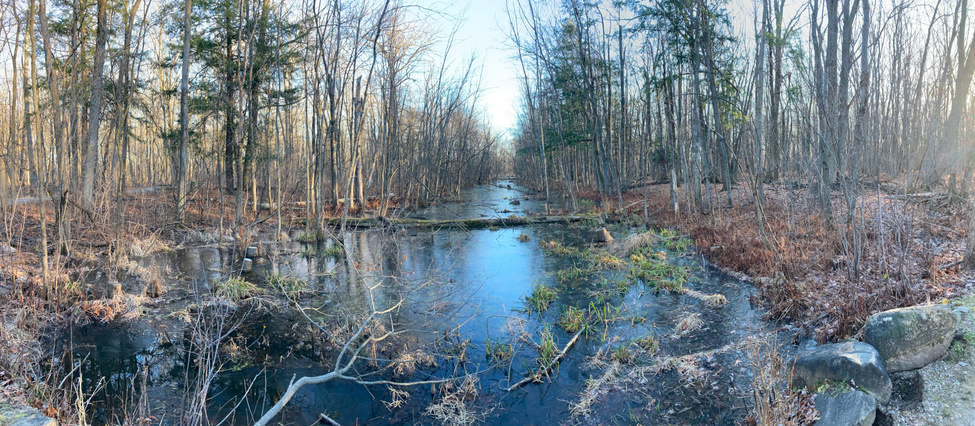
\includegraphics[width=7in]{images/cover_nature5_xs}}
%    \newsavebox{\coverwindmill}
%    \savebox{\coverwindmill}{\includegraphics[width=2in]{images/cover_windmill}}
    \newsavebox{\telescope}
    \savebox{\telescope}{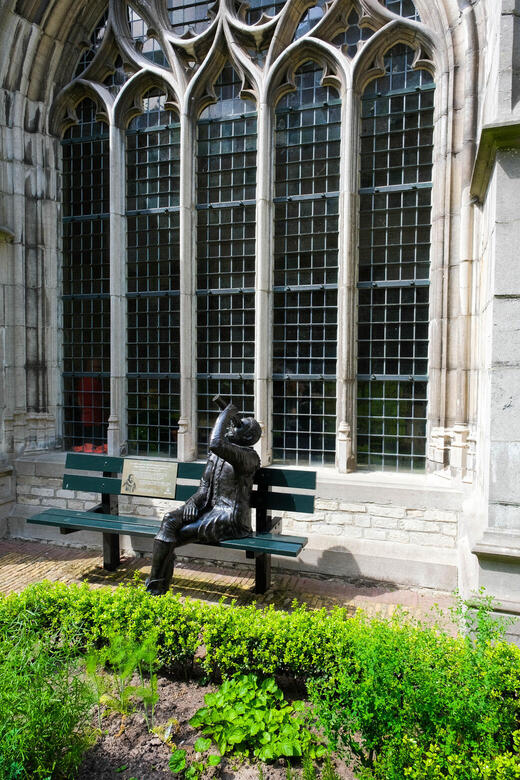
\includegraphics[width=2.5in]{images/cover_telescope}}
    \begin{inctext}[paper=current, target=mytarget]
      \begin{tikzpicture}
        \coordinate (A) at (0,0);
        \coordinate (B) at (8.5in,11in);
        \fill[use as bounding box,color=red!5] (A) rectangle (B);
        \coordinate (C) at ([xshift=0.5in,yshift=0.5in]A);
        \coordinate (D) at ([xshift=-0.5in,yshift=-0.5in]B);
        \draw[rounded corners=0.25in,very thick,black] (C) rectangle (D);
        \node[inner sep=0pt,above right] (nature5) at (0.75in,2.5in) {\usebox{\covernature}};
        \fill[red!5,path fading=south] (0.75in,4.8in) rectangle (7.75in,5.6in);
        \node[inner sep=0pt,below right] (telescope) at (0.75in,10in) {\usebox{\telescope}};
        \fill[red!5,path fading=north] (0.75in,6.2in) rectangle (3.26in,7in);
        \fill[red!5,path fading=west] (3in,6.2in) rectangle (3.26in,10in);
        \node[text width=10cm,align=flush center,font=\Huge\bfseries] at (5.5in,8in) {\UOtitle};
        \node[inner sep=0pt,above right] (UOlogo) at (1in,1in) {\includegraphics[width=\UOlogoCLopt]{\UOlogoCLloc}};
        \node[text width=6cm,above left,font=\large\bfseries] (author) at (7.5in,1in) {\UOauthor \\ \UO};
      \end{tikzpicture}
    \end{inctext}
  \end{titlepage}
  \pagecolor{white}
  \clearemptydoublepage
}

%%%%%%%%%%%%%%%%%%%%%%%%%%%%%%%%%%%%%%%%%%%%%%%%%%%%%%%%%%%%%%%%%%%%%%
% The open source page
%%%%%%%%%%%%%%%%%%%%%%%%%%%%%%%%%%%%%%%%%%%%%%%%%%%%%%%%%%%%%%%%%%%%%%
\newcommand{\UOopenloc}{images/open_source}     % Location of the logo
\newcommand{\UOopenopt}{2cm}             % Options for includegraphics

\newcommand{\opensource}{
  \thispagestyle{empty}

  \noindent \copyright\ \UOauthor, \UOyear\ (\UO)
  
  \noindent Version adapt\'ee de {\it Calcul diff\'erentiel et
  int\'egral pour les sciences de la vie}, manuel pour les cours MAT1730
  et MAT1732, et des notes pour les cours MAT1720, MAT1722 et MAT2722
  de calcul diff\'erentiel et int\'egral pour l'ing\'enierie.

  \noindent Ce document est disponible aux endroits suivants :\\
  Recherche uO: http://hdl.handle.net/10393/44594 \\
  GitHub: https://github.com/BenoitDionne/Calculus

  \vspace*{1cm}
  
  \noindent \includegraphics[width=\UOopenopt]{\UOopenloc}

  \noindent Sauf indication contraire, ce livre est mis \`a disposition selon
  les termes de la licence \href{https://creativecommons.org/licenses/by-nc-sa/4.0/deed.fr}{Creative Commons Attribution - Pas d’Utilisation Commerciale - Partage dans les M\^emes Conditions 4.0 International} (CC BY-NC-SA 4.0)

  \vfill

  \noindent Page couverture:\\
  Statue de Hans Lipperhey, Pays-Bas, 1570-1619, photo par Louise Oegema.\\
  Un \'etang, photo par Patrice Dionne.

  \noindent Entêtes des chapitres:\\
  Les images utilis\'ees pour les ent\^ees des chapitres sont quelques
  unes des illustrations produites par John Tenniel pour la version
  originale du livre {\bfseries Alice's Adventures in Wonderland} par
  Lewis Carroll.

  \clearemptydoublepage
}

%%%%%%%%%%%%%%%%%%%%%%%%%%%%%%%%%%%%%%%%%%%%%%%%%%%%%%%%%%%%%%%%%%%%%%
% The bibliography
%%%%%%%%%%%%%%%%%%%%%%%%%%%%%%%%%%%%%%%%%%%%%%%%%%%%%%%%%%%%%%%%%%%%%%
\newcommand{\UObibliography}{
  \setcounter{chapter}{100}
  \addcontentsline{toc}{chapter}{Bibliographie}
  \begin{thebibliography}{99}

\bibitem{A} F.\ R.\ Adler, {\bfseries Modeling the Dynamics of Life:
Calculus and Probability for Life Scientists}, Brooks/Cole, 2005.

\bibitem{BE} D. Betounes, {\bfseries Partial Differential Equations for
Computational Science}, Springer-Verlag, 1998.

\bibitem{BC} R. L. Borelli et C. S. Coleman,
{\bfseries Differential Equations, a Modeling Perspective}, Wiley, 1998.

\bibitem{BR} M. Braun, {\bfseries Differential Equations and their
Applications, 4$^{th}$ edition}, Springer-Verlag, 1993.

\bibitem{LC} L. Carroll, {\bfseries Alice's Adventures in Wonderland},

\bibitem{FL} G. B. Folland, {\bfseries Advanced Calculus}, Prentice Hall, 2002

\bibitem{I} R. Illner, C. S. Bohun, S. McCollum et T. an Roode,
{\bfseries Mathemtical Modelling: A Case Studies Approach}, AMS, 2005.

\bibitem{SL} S. Lipschutz, {\bfseries Linear Alegebra}, Schaum's Outline
  Series, McGraw-Hill, 1968.

\bibitem{MT} J. E. Marsden and A. J. Tromba, {\bfseries Vector
 Calculus, 2$^{nd}$ edition}, W. H. Freedman and Company, 1981.

\bibitem{M} J. D. Murray, {\bfseries Mathematical Biology, 1: An
Introduction, 3$^{th}$ edition}, Springer-Verlag, 2002.

\bibitem{NH} C. Newhouser, {\bfseries Calculus for Biology and
Medecine 2$^{nd}$ Edition}, Prentice Hall, 2004

\bibitem{ND} B. Noble and J. W. Daniel, {\bfseries Applied Linear Algebra},
3$^{rd}$ edition, Prentice-Hall, 1988.

\bibitem{O} M. Olinick, {\bfseries An Introduction to Mathematical Models in
the Social and Life Sciences}, Addison-Wesley, 1978

\bibitem{R} D. A. Roff, {\bfseries The Evolution of Life Histories},
Chapman and Hall, 1992

\end{thebibliography}

%%% Local Variables: 
%%% mode: latex
%%% TeX-master: "notes"
%%% End:

  \clearemptydoublepage
}

%%%%%%%%%%%%%%%%%%%%%%%%%%%%%%%%%%%%%%%%%%%%%%%%%%%%%%%%%%%%%%%%%%%%%%
% List of tables and figures
%%%%%%%%%%%%%%%%%%%%%%%%%%%%%%%%%%%%%%%%%%%%%%%%%%%%%%%%%%%%%%%%%%%%%%
\newcommand{\UOtablesfigureslist}{
  \addcontentsline{toc}{chapter}{\LofT}
  \listoftables
  \clearemptydoublepage

  \addcontentsline{toc}{chapter}{\LofF}
  \listoffigures
  \clearemptydoublepage
}

%%%%%%%%%%%%%%%%%%%%%%%%%%%%%%%%%%%%%%%%%%%%%%%%%%%%%%%%%%%%%%%%%%%%%%
% graphics, ...
%%%%%%%%%%%%%%%%%%%%%%%%%%%%%%%%%%%%%%%%%%%%%%%%%%%%%%%%%%%%%%%%%%%%%%
\usepackage{graphicx}
\usepackage{rotating}    % To rotate figures, tables, ...
\usepackage{color}
\usepackage{subfig}

% By default figures will be placed "here" if possible otherwise at
% the "top."
\makeatletter
\renewcommand*{\fps@figure}{ht}
\makeatother

% Methods for figures.
\newcommand{\PDFfig}[5][TTT]{%
  \ifthenelse{\equal{TTT}{#1}}{\begin{figure}}{\begin{figure}[#1]}%
      {\color{purple}\rule{\textwidth}{1pt}}\begin{center}%
        \input{#2.pdf_t}\end{center}\caption[#3]{#4 \label{#5}}%
      {\color{purple}\rule{\textwidth}{1pt}}%
    \end{figure}}

\newcommand{\PDFfigD}[6][TTT]{
  \ifthenelse{\equal{TTT}{#1}}{\begin{figure}}{\begin{figure}[#1]}%
      {\color{purple}\rule{\textwidth}{1pt}}\begin{center} %
        \input{#2.pdf_t}\end{center} %
      \begin{center}\input{#3.pdf_t}\end{center} %
      \caption[#4]{#5 \label{#6}}%
      {\color{purple}\rule{\textwidth}{1pt}}%
    \end{figure}}

\newcommand{\PDFfigR}[5]{\begin{figure}%
    {\color{purple}\rule{\textwidth}{1pt}}\begin{center}
      \resizebox{#2}{!}{\input{#1.pdf_t}}\end{center}
    \caption[#3]{#4 \label{#5}}%
    {\color{purple}\rule{\textwidth}{1pt}}\end{figure}}

\newcommand{\PDFgraph}[1]{\begin{center}\input{#1.pdf_t}\end{center}}

\newcommand{\PDFgraphRow}[2]{\raisebox{#2}{\input{#1.pdf_t}}}

\newcommand{\MATHfig}[6][TTT]{%
  \ifthenelse{\equal{TTT}{#1}}{\begin{figure}}{\begin{figure}[#1]}%
      {\color{purple}\rule{\textwidth}{1pt}}\begin{center} %
        \includegraphics[width=#3]{#2}\end{center} %
      \caption[#4]{#5 \label{#6}}%
      {\color{purple}\rule{\textwidth}{1pt}}%
    \end{figure}}

\newcommand{\MATHfigD}[7]{\begin{figure}%
    {\color{purple}\rule{\textwidth}{1pt}}\begin{center}%
      \includegraphics[width=#2]{#1}\includegraphics[width=#4]{#3}\end{center}%
    \caption[#5]{#6 \label{#7}}%
    {\color{purple}\rule{\textwidth}{1pt}}\end{figure}}

\newcommand{\MATHgraph}[2]{\begin{center}%
    \includegraphics[width=#2]{#1}\end{center}}

\newcommand{\MATHgraphRow}[3]{\raisebox{#3}{\includegraphics[width=#2]{#1}}}

%%%%%%%%%%%%%%%%%%%%%%%%%%%%%%%%%%%%

% Methods for eps Figures.
\newcommand{\epsF}[5]{\begin{figure}\begin{center} %
\includegraphics[width=#2]{#1}\end{center} %
\caption[#3]{#4 \label{#5}}\end{figure}}

\newcommand{\epsD}[7]{\begin{figure}\begin{center} %
\includegraphics[width=#2]{#1}\includegraphics[width=#4]{#3}\end{center} %
\caption[#5]{#6 \label{#7}}\end{figure}}

\newcommand{\epsbox}[2]{\begin{center}%
\includegraphics[width=#2]{#1}\end{center}}

% Methods for pstex Figures.
\newcommand{\pstexF}[4]{\begin{figure}\begin{center} %
\input{#1.pstex_t}\end{center}\caption[#2]{#3 \label{#4}}\end{figure}}

\newcommand{\figbox}[1]{\begin{center}\input{#1.pstex_t}\end{center}}

\newcommand{\pstexD}[5]{\begin{figure}\begin{center} %
\input{#1.pstex_t}\end{center} %
\begin{center}\input{#2.pstex_t}\end{center} %
\caption[#3]{#4 \label{#5}}\end{figure}}

\newcommand{\pstexR}[5]{\begin{figure}\begin{center}
\resizebox{#2}{!}{\input{#1.pstex_t}}\end{center}
\caption[#3]{#4 \label{#5}}\end{figure}}

%%%%%%%%%%%%%%%%%%%%%%%%%%%%%%%%%%%%%%%%%%%%%%%%%%%%%%%%%%%%%%%%%%%%%%
% Formats for the remarks, examples, ...
%%%%%%%%%%%%%%%%%%%%%%%%%%%%%%%%%%%%%%%%%%%%%%%%%%%%%%%%%%%%%%%%%%%%%%
\makeatletter

\newcommand{\rmk@one}[1][RRR]{\def\argrmk@one{#1}\rmk@two}

\newcommand{\rmk@two}[1][TTT]%
{\refstepcounter{focus}\renewcommand{\labelitemi}{\textbullet}%
  \noindent {\bfseries Remarque \thefocus}%
  \ifthenelse{\equal{TTT}{#1}}{}{\ ({\bfseries #1})}%
  \ifthenelse{\equal{RRR}{\argrmk@one}}{\\ \noindent}%
  {\ \argrmk@one \\ \noindent}%
}

\newenvironment{rmk}{\rmk@one}{\hspace*{\fill} $\spadesuit$}

\newcommand{\rmkList@one}[1][RRR]{\def\argrmk@one{#1}\rmkList@two}

\newcommand{\rmkList@two}[1][TTT]%
{\refstepcounter{focus}\renewcommand{\labelitemi}{\textbullet}%
  \noindent {\bfseries Remarque \thefocus}%
  \ifthenelse{\equal{TTT}{#1}}{}{\ ({\bfseries #1})}%
  \ifthenelse{\equal{RRR}{\argrmk@one}}{\\ \vspace*{-1\topskip}\noindent}%
  {\ \argrmk@one \\ \vspace*{-1\topskip}\noindent}%
}

\newenvironment{rmkList}{\rmkList@one}{\hspace*{\fill} $\spadesuit$}

\newcommand{\egg@one}[1][RRR]{\def\argegg@one{#1}\egg@two}

\newcommand{\egg@two}[1][TTT]%
{\refstepcounter{focus}\renewcommand{\labelitemi}{\textbullet}%
  \noindent {\bfseries Exemple \thefocus}%
  \ifthenelse{\equal{TTT}{#1}}{}{\ ({\bfseries #1})}%
  \ifthenelse{\equal{RRR}{\argegg@one}}{\\ \noindent}%
  {\ \argegg@one \\ \noindent}%
}

\newenvironment{egg}{\egg@one}{\hspace*{\fill} $\clubsuit$}

\makeatother

% Title for the multiple choices, the parts of a proof, etc.
\newcommand{\subQ}[1]{\noindent {\bfseries #1})\ }
\newcommand{\subI}[1]{\noindent {\bfseries #1}:\ }
\newcommand{\solTitle}{\noindent {\bfseries Solution:}\\}

%%%%%%%%%%%%%%%%%%%%%%%%%%%%%%%%%%%%%%%%%%%%%%%%%%%%%%%%%%%%%%%%%%%%%%
% Mathematical symbols, short cuts, ...
%%%%%%%%%%%%%%%%%%%%%%%%%%%%%%%%%%%%%%%%%%%%%%%%%%%%%%%%%%%%%%%%%%%%%%
\newcommand{\NN}{\mathbb{N}}
\newcommand{\NNp}{\mathbb{N}^+}
\newcommand{\ZZ}{\mathbb{Z}}
\newcommand{\RR}{\mathbb{R}}
\newcommand{\QQ}{\mathbb{Q}}
\newcommand{\CC}{\mathbb{C}}
\newcommand{\OO}{\mathcal{O}}
\newcommand{\FF}{\mathcal{F}}

\newcommand{\ps}[2]{ \left\langle{#1} , {#2}\right\rangle }
\newcommand{\VEC}[1]{\mathbf{#1}}
\newcommand{\SN}[1]{\mathrm{S}_{#1}}
\newcommand{\sgm}[1]{\overline{#1}}
\newcommand{\ii}{\VEC{i}}
\newcommand{\jj}{\VEC{j}}
\newcommand{\kk}{\VEC{k}}
\newcommand{\nn}{$n\times n$\ }
\newcommand{\nm}[2]{${#1}\times {#2}$\ }

\DeclareMathOperator{\IM}{Im\ }
\DeclareMathOperator{\DO}{Dom\ }
\DeclareMathOperator{\arcsec}{arcsec}
\DeclareMathOperator{\tr}{tr}
\DeclareMathOperator{\Id}{I}   % ou Id  ?
\DeclareMathOperator{\sgn}{sgn}
\DeclareMathOperator{\curl}{rot}
\DeclareMathOperator{\diV}{div}
\DeclareMathOperator{\graD}{grad}
\DeclareMathOperator{\sech}{sech}
\DeclareMathOperator{\csch}{csch}

\newcommand{\diff}{\mathrm{D}}
\newcommand{\dx}[1]{\,\mathrm{d}#1}
\newcommand{\dydx}[2]{\frac{\mathrm{d}#1}{\mathrm{d}#2}}
\newcommand{\dydxn}[3]{\frac{\mathrm{d}^{#3}#1}{\mathrm{d}#2^{#3}}}
\newcommand{\dfdx}[2]{\frac{\mathrm{d}}{\mathrm{d}#2}#1}
\newcommand{\dfdxn}[3]{\frac{\mathrm{d}^{#3}}{\mathrm{d}#2^{#3}}#1}

\newcommand{\pdydx}[2]{\frac{\partial #1}{\partial #2}}
\newcommand{\pdydxn}[3]{\frac{\partial^{#3} #1}{\partial #2^{#3}}}
\newcommand{\pdydxnm}[6]{\frac{\partial^{#4} #1}%
{\partial #2^{#5} \partial #3^{#6}}}

\newcommand{\pdfdx}[2]{\frac{\partial}{\partial #2} #1}
\newcommand{\pdfdxn}[3]{\frac{\partial^{#3}}{\partial #2^{#3}} #1}
\newcommand{\pdfdxnm}[6]{\frac{\partial^{#4}}%
{\partial #2^{#5} \partial #3^{#6}} #1}

\newcommand{\Maug}[2]{\left(\begin{array}{c|c}{#1}&{#2}\end{array}\right)}

\newcommand{\rectangle}{
%\begin{tikzpicture}
\tikz \draw (0,0) rectangle (0.4,0.3);
%\end{tikzpicture}
}

\newcommand{\trapeze}{
%\begin{tikzpicture}
\tikz \draw (0,0) -- (0.2,0.3) -- (0.5,0.3) -- (0.3,0) -- cycle;
%\end{tikzpicture}
}

\renewcommand{\qed}{\hfill \mbox{\raggedright \rule{0.4em}{0.8em}}\\[1em]}

\makeatletter

\newcommand{\proof@one}[1][RRR]{\def\argproof@one{#1}\proof@two}

\newcommand{\proof@two}[1][TTT]%
{\noindent\textbf{\UOproof}\ %
  \ifthenelse{\equal{TTT}{#1}}{}{\ ({\bfseries #1})} %
  \ifthenelse{\equal{RRR}{\argproof@one}}{\\ \noindent}%
  {\ \argproof@one \\ \noindent}%
  \normalfont%
}

\renewenvironment{proof}{\proof@one}{\hspace*{\fill} \qed}

\makeatother

%%%%%%%%%%%%%%%%%%%%%%%%%%%%%%%%%%%%%%%%%%%%%%%%%%%%%%%%%%%%%%%%%%%%%%
% To produce assignments and the solutions for the problems of a
% chapter
%%%%%%%%%%%%%%%%%%%%%%%%%%%%%%%%%%%%%%%%%%%%%%%%%%%%%%%%%%%%%%%%%%%%%%
\newcounter{questNBR}[chapter]
\renewcommand\thequestNBR{\thechapter.\arabic{questNBR}}

\makeatletter

\newcommand{\quest@one}[1][RRR]{\def\argquest@one{#1}\quest@two}

\newcommand{\quest@two}[1][TTT]%
{\refstepcounter{questNBR}\noindent%
  {\bfseries Question \arabic{chapter}.\arabic{questNBR}}%
  \ifthenelse{\equal{TTT}{#1}}{}{\ ({\bfseries #1})}%
  \ifthenelse{\equal{RRR}{\argquest@one}}{\\ \noindent}{\ \argquest@one \\ \noindent}%
}

\newenvironment{question}{\quest@one}{}

\makeatother

%%%%%%%%%%%%%%%%%%%%%%%%%%%%%%%%%%%%%%%%%%%%%%%%%%%%%%%%%%%%%%%%%%%%%%
% The index
%%%%%%%%%%%%%%%%%%%%%%%%%%%%%%%%%%%%%%%%%%%%%%%%%%%%%%%%%%%%%%%%%%%%%%
\usepackage{makeidx}
\makeindex
\newcommand{\UOindex}{
  \setcounter{chapter}{100}
  \addcontentsline{toc}{chapter}{\indexname}
  \printindex
}

%%%%%%%%%%%%%%%%%%%%%%%%%%%%%%%%%%%%%%%%%%%%%%%%%%%%%%%%%%%%%%%%%%%%%% 
% Sometime useful
%%%%%%%%%%%%%%%%%%%%%%%%%%%%%%%%%%%%%%%%%%%%%%%%%%%%%%%%%%%%%%%%%%%%%%
\usepackage{multicol}

%%%%%%%%%%%%%%%%%%%%%%%%%%%%%%%%%%%%%%%%%%%%%%%%%%%%%%%%%%%%%%%%%%%%%%
% Extra fonts of the form  \fa...
%%%%%%%%%%%%%%%%%%%%%%%%%%%%%%%%%%%%%%%%%%%%%%%%%%%%%%%%%%%%%%%%%%%%%%
\usepackage{fontawesome}

%%%%%%%%%%%%%%%%%%%%%%%%%%%%%%%%%%%%%%%%%%%%%%%%%%%%%%%%%%%%%%%%%%%%%%
% Formatting of the notes
%%%%%%%%%%%%%%%%%%%%%%%%%%%%%%%%%%%%%%%%%%%%%%%%%%%%%%%%%%%%%%%%%%%%%%
\newboolean{THEO}
\setboolean{THEO}{false}
\newcommand{\setTHEO}{\setboolean{THEO}{true}}

\newcommand{\compileTHEO}[1]{
  \ifthenelse{\boolean{THEO}}{#1}{}
}

\newcommand{\SOLUa}{hide}
\newcommand{\setSOLUa}{\renewcommand{\SOLUa}{show}}

\newcommand{\SOLUb}{hide}
\newcommand{\setSOLUb}{\renewcommand{\SOLUb}{show}}

\newcommand{\SOLUc}{hide}
\newcommand{\setSOLUc}{\renewcommand{\SOLUc}{show}}

% \newcommand{\compileSOL}[3]{
% \ifthenelse{\equal{#1}{show}}{{\bfseries\noindent Question~#2}\\ #3}{\ \newline\newline}
% }

\newenvironment{SOLUTION}{}{}
\newcommand{\compileSOL}[3]{
\ifthenelse{\equal{#1}{show}}{
\begin{SOLUTION}
{\bfseries\noindent Question~#2}\\ #3
\end{SOLUTION}
}{}}

\newcommand{\compileSOLU}[2]{
  \ifthenelse{\equal{#1}{show}}{\solTitle #2}{}
}

\newcommand{\HIDE}{show}
\newcommand{\setHIDE}{\renewcommand{\HIDE}{hide}}

\newcommand{\compileText}[2]{
  \ifthenelse{\equal{#1}{hide}}{}{#2}
}

% Many solutions use  \compileText{solOUT}{}{}  because we
% didn't want to print them.

\newcommand{\theory}{\faEye\ }
\newcommand{\eng}{\faWrench\ }
\newcommand{\eco}{\faLineChart\ }
\newcommand{\life}{\faTree\ }
